\documentclass[10pt,a4paper]{article}
\usepackage[utf8]{inputenc}
\usepackage[T1]{fontenc}
\usepackage[spanish,es-tabla]{babel}
\usepackage{lmodern}
\usepackage{amsmath,amssymb}
\usepackage[margin=1.65cm,top=1.65cm,bottom=1.55cm]{geometry}
\usepackage{graphicx}
\usepackage{caption}
\usepackage{microtype}
\usepackage{booktabs}
\usepackage{xcolor}
\usepackage{hyperref}
\hypersetup{colorlinks=true,allcolors=blue!50!black}
\captionsetup{font=footnotesize,labelfont=bf,skip=3pt}
\setlength{\parindent}{0.8em}
\setlength{\parskip}{2pt}
\renewcommand{\baselinestretch}{1.03}
\newcommand{\vf}{\boldsymbol{Y}}
\begin{document}
\begin{center}
{\Large\bfseries Simulación numérica del modelo de neuronas de Izhikevich}\\[4pt]
{\normalsize Tomás Navarro Febre}\\[2pt]
{\small Fundamentos de Redes Neuronales --- Trabajo Práctico 1, 2026}
\end{center}
\vspace{-6pt}
\section*{Resumen}
Estudiamos numéricamente el modelo de disparo de Izhikevich mediante Runge--Kutta de cuarto orden (RK4) y reseteo discreto tras cada paso. Se reproducen ocho patrones neuronales, incluidas adaptación, ráfagas, rebote y resonancia, y se contrasta la sensibilidad a la discretización. Una red heterogénea de 1000 neuronas, simulada con el esquema del artículo original, exhibe disparos mayormente asincrónicos y episodios de sincronización. La eliminación de autoconexiones modifica moderadamente su tasa de disparo. Finalmente, integramos una neurona con ruido blanco mediante Euler--Maruyama y comparamos diferentes realizaciones con un control determinista.

\section{Introducción y modelo}
El modelo de Izhikevich proporciona actividad neuronal compleja con sólo dos variables dinámicas; su eficiencia posibilita pasar de células individuales a redes grandes sin resolver modelos iónicos de Hodgkin--Huxley \cite{izhikevich,hodgkin}. Nuestro objetivo es reconstruir las dinámicas de las Figs.~2 y 3 de \cite{izhikevich} siguiendo los protocolos del TP1.
\begin{equation}
\dot v=0.04v^2+5v+140-u+I(t),\qquad \dot u=a(bv-u),\label{eq:modelo}
\end{equation}
con el \emph{reseteo} $v\leftarrow c,\ u\leftarrow u+d$ cuando el algoritmo detecta $v\geq30$ mV. El potencial $v$ y la variable de recuperación $u$ representan respectivamente la excitación y la realimentación lenta; $I$ es la corriente efectiva, $a$ y $b$ determinan la dinámica de recuperación y $c,d$ los saltos tras disparar. \emph{Los $30$ mV registran el máximo del spike, no un umbral fisiológico fijo.}

\section{Neurona individual y estímulo escalón}
Usamos $a=0.02$, $b=0.2$, $c=-65$, $d=2$, $v(0)=-70$ mV, $u(0)=-14$, $h=0.1$ ms, e $I=10$ para $t\geq10$ ms (cero antes). Se emplea \texttt{paso\_rk4} del integrador del repositorio, seguido por detección y reseteo. La Fig.~\ref{fig:base} muestra siete disparos en $100$ ms; el primero sucede a $13.5$ ms. Los intervalos entre disparos crecen al principio y $u$ aumenta con cada evento, consistente con la retroalimentación adaptativa.
\begin{figure}[h!]
\centering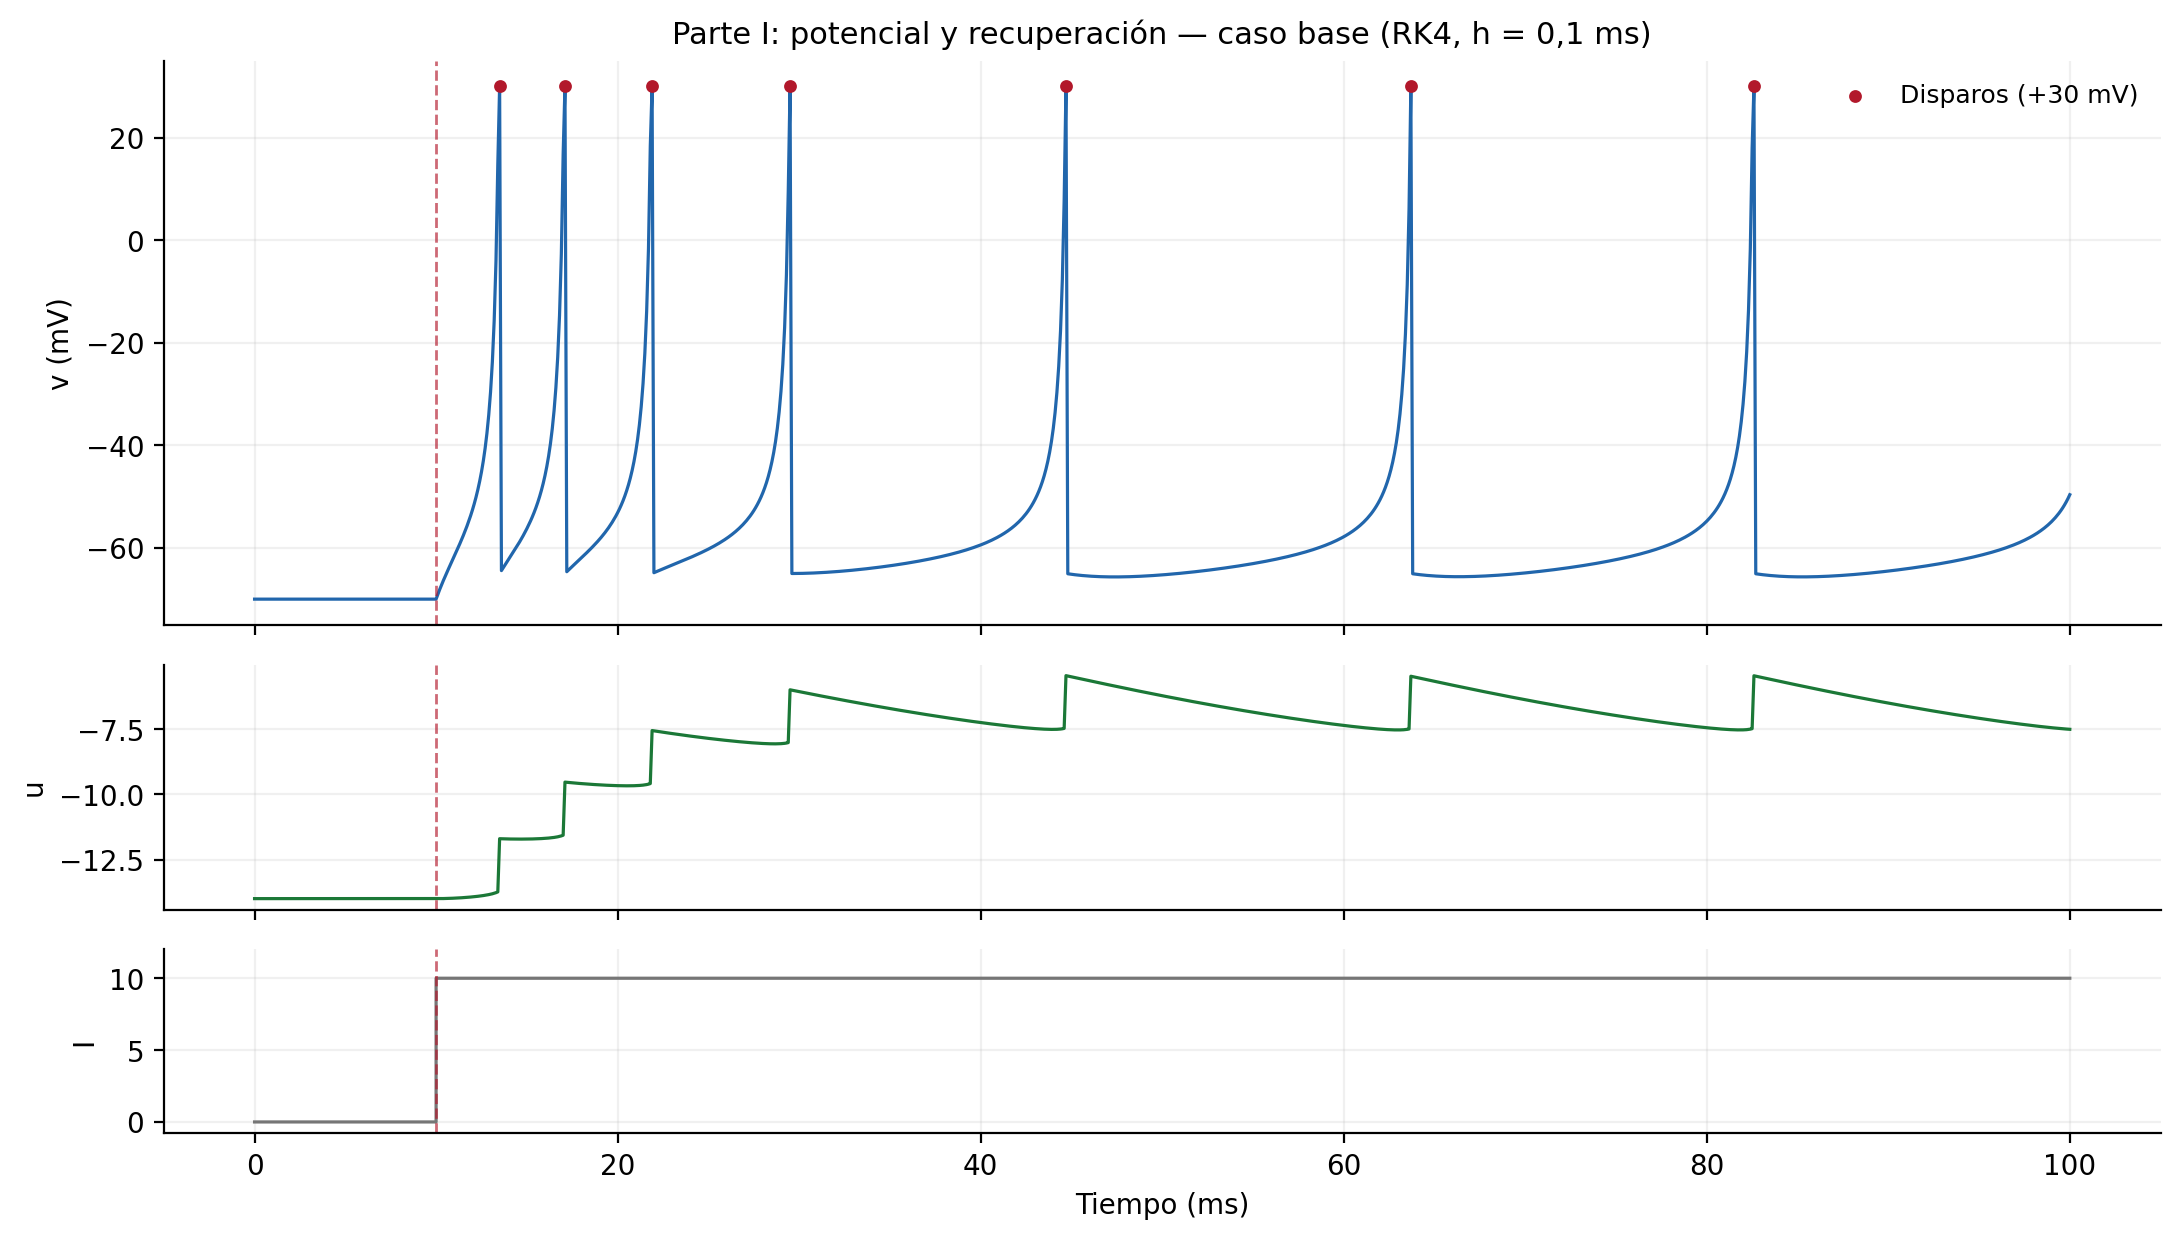
\includegraphics[width=0.89\linewidth]{../figuras/01_caso_base.png}
\caption{Caso base: $v(t)$, $u(t)$ y corriente aplicada. La línea punteada indica el inicio del estímulo; los puntos a $30$ mV son registros discretos de eventos.}\label{fig:base}
\end{figure}
\newpage
\section{Ocho regímenes de disparo}
La Fig.~\ref{fig:tipos} reproduce los ocho casos pedidos. Se mantuvo $h=0.1$ ms y se usaron los parámetros y protocolos explícitos del enunciado, incluyendo pulsos negativos para TC2 y un pulso de conmutación para RZ. En cada panel la curva azul es el potencial y la roja la entrada aplicada (escala derecha).
\begin{figure}[h!]
\centering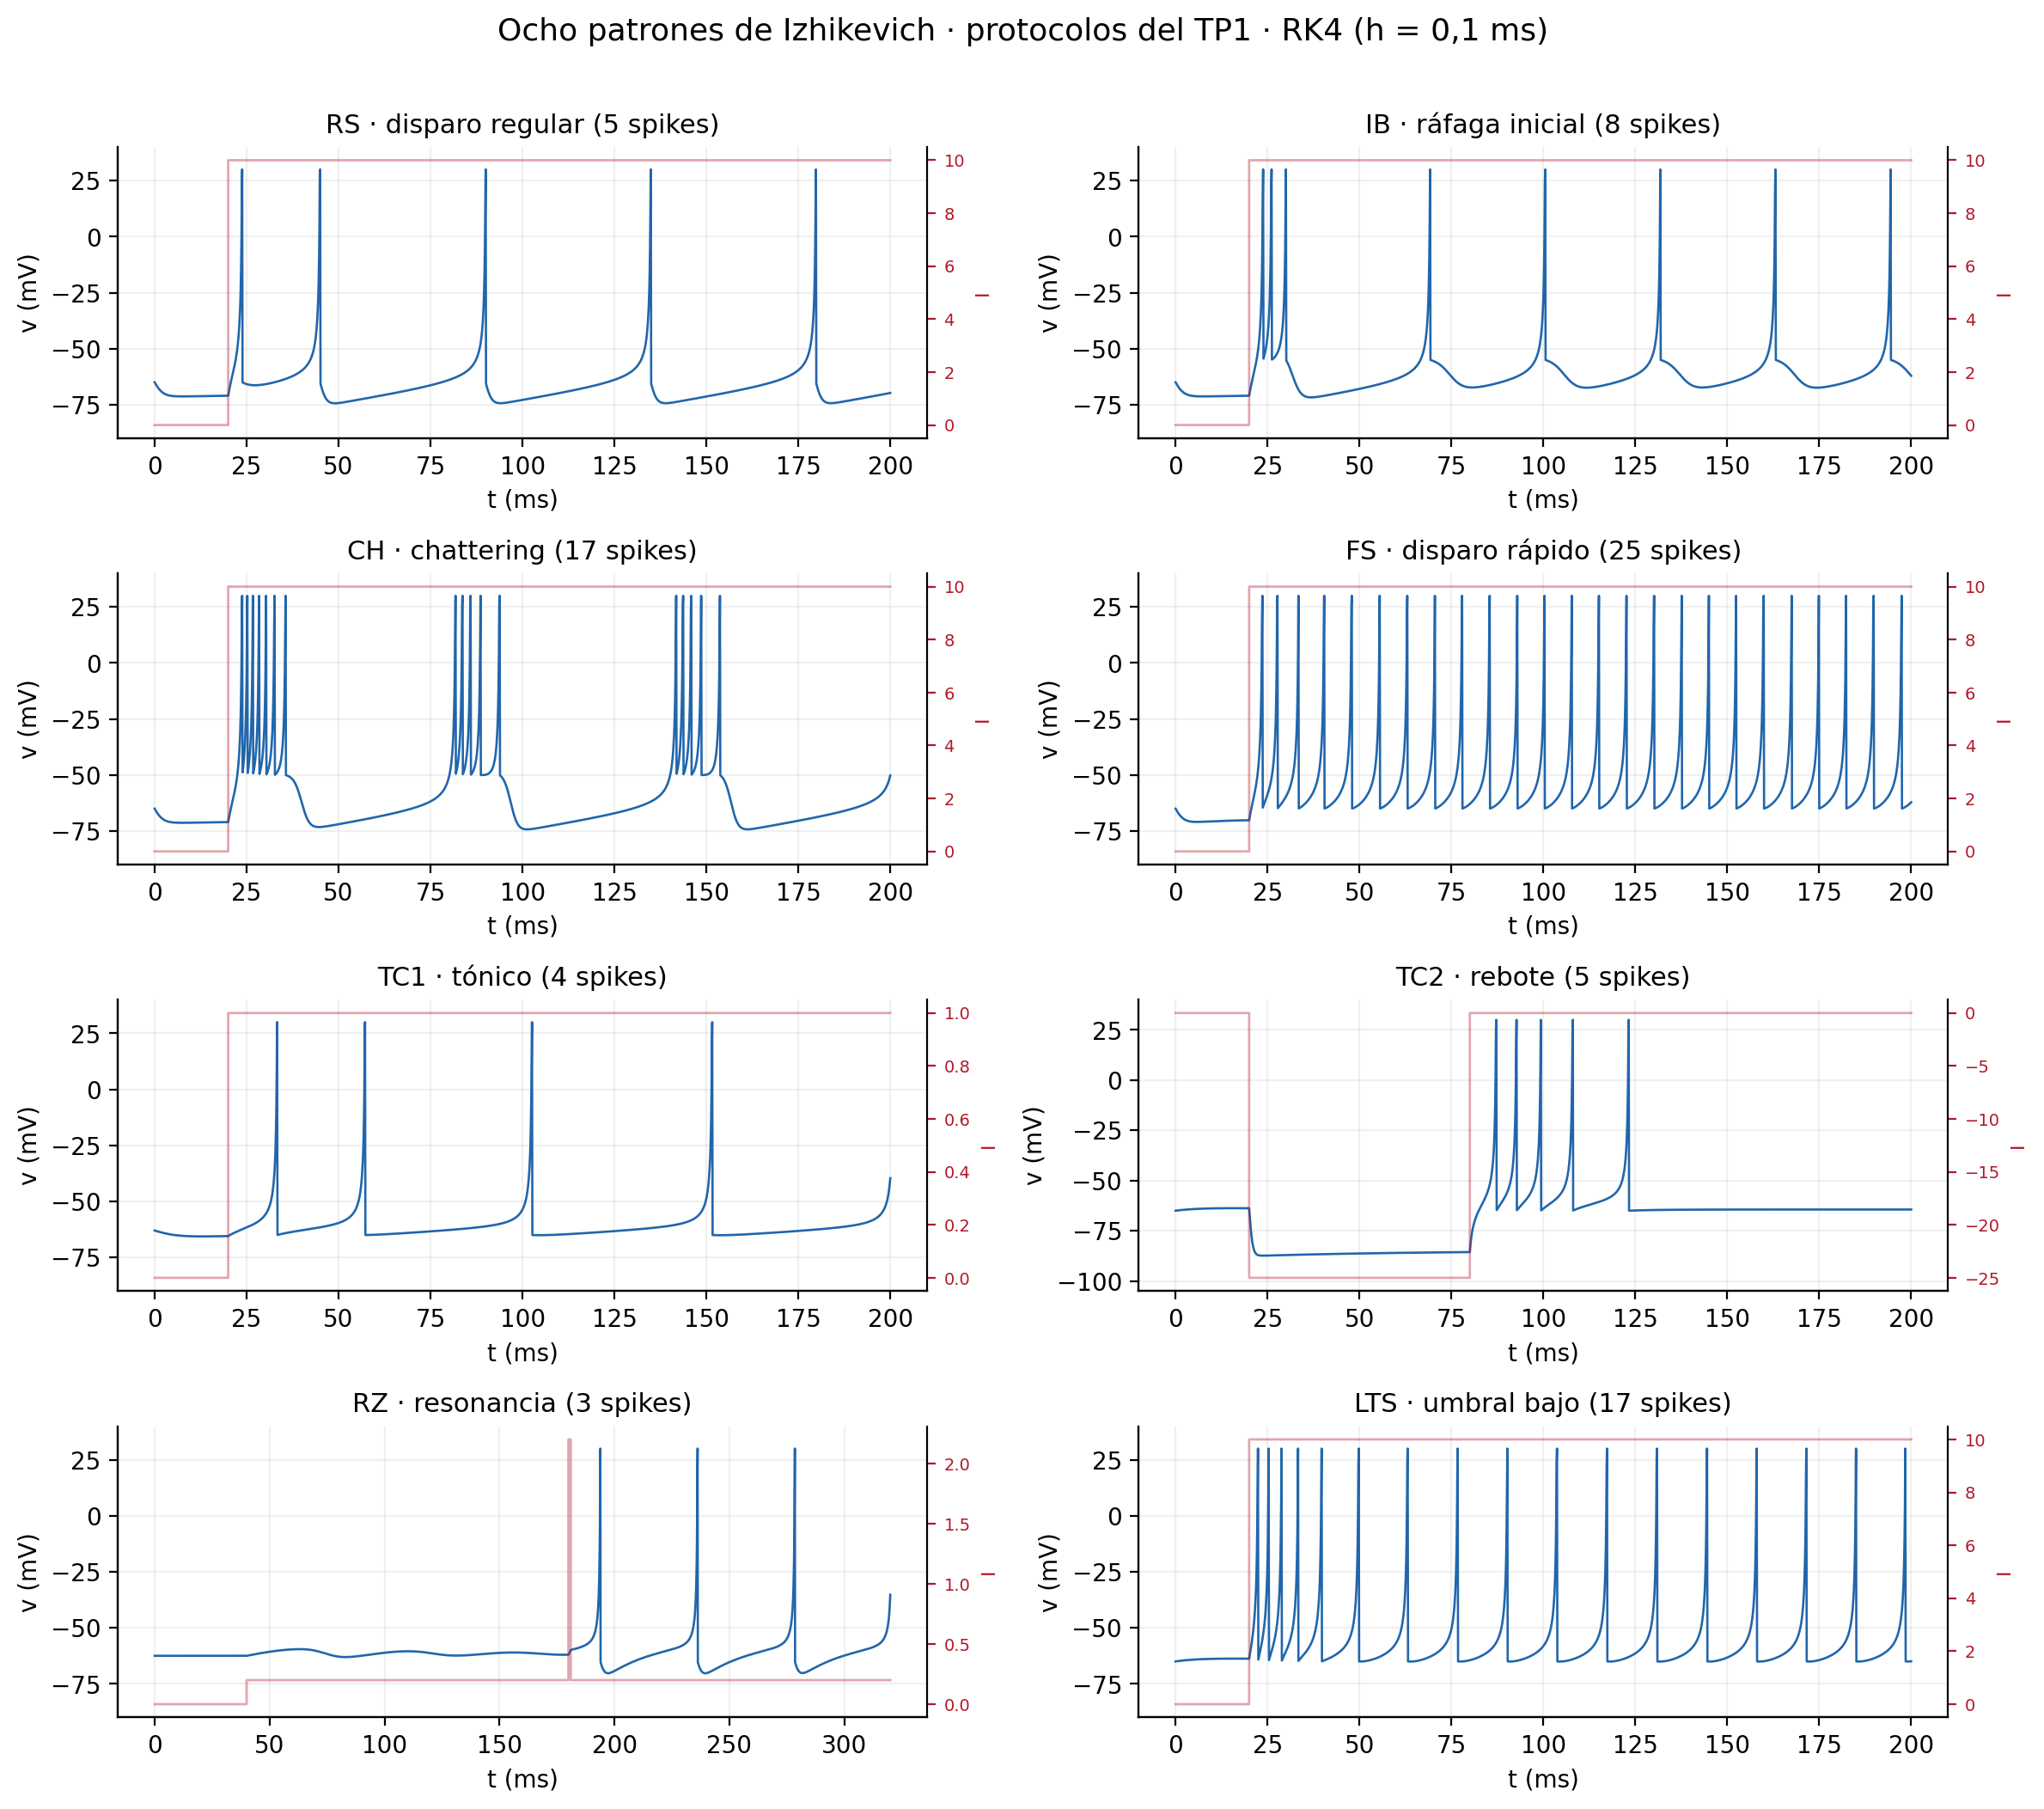
\includegraphics[width=0.85\linewidth]{../figuras/02_ocho_tipos.png}
\caption{Dinámicas RS, IB, CH, FS, TC1, TC2, RZ y LTS, comparables cualitativamente con la Fig.~2 de Izhikevich \cite{izhikevich}.}\label{fig:tipos}
\end{figure}
\vspace{-3pt}
\textbf{Interpretación.} RS presenta adaptación de frecuencia; IB, una ráfaga inicial antes de disparos aislados; CH, grupos repetidos de spikes densos; FS, disparos frecuentes con adaptación escasa. TC1 dispara tónicamente desde reposo y TC2 produce una ráfaga de rebote al retirar la hiperpolarización. RZ exhibe oscilación subumbral y pasa a disparar tras el pulso breve; LTS muestra numerosos disparos y adaptación. Los ocho regímenes coinciden cualitativamente con los del artículo, aunque las amplitudes y los tiempos de TC/RZ provienen del TP, no de una tabla experimental de \cite{izhikevich}.
\newpage
\section{Red de 1000 neuronas}
Se reproduce la Sección IV de \cite{izhikevich}: $N_E=800$, $N_I=200$, parámetros heterogéneos, pesos aleatorios $S=[0.5R_E\mid-R_I]$ y entrada talámica gaussiana renovada \emph{cada milisegundo} ($5\xi$ en excitatorias, $2\xi$ en inhibitorias). El acoplamiento es por pulsos: $I_i^{\mathrm{sin}}=\sum_{j\in F}s_{ij}$ con $F=\{j:v_j\ge30\}$. Se siguió el código Matlab original: dos actualizaciones de Euler de $0.5$ ms para $v$ y una de $1$ ms para $u$, con detección al principio del paso de $1$ ms. Semilla: \textbf{2026}.
\begin{figure}[h!]
\centering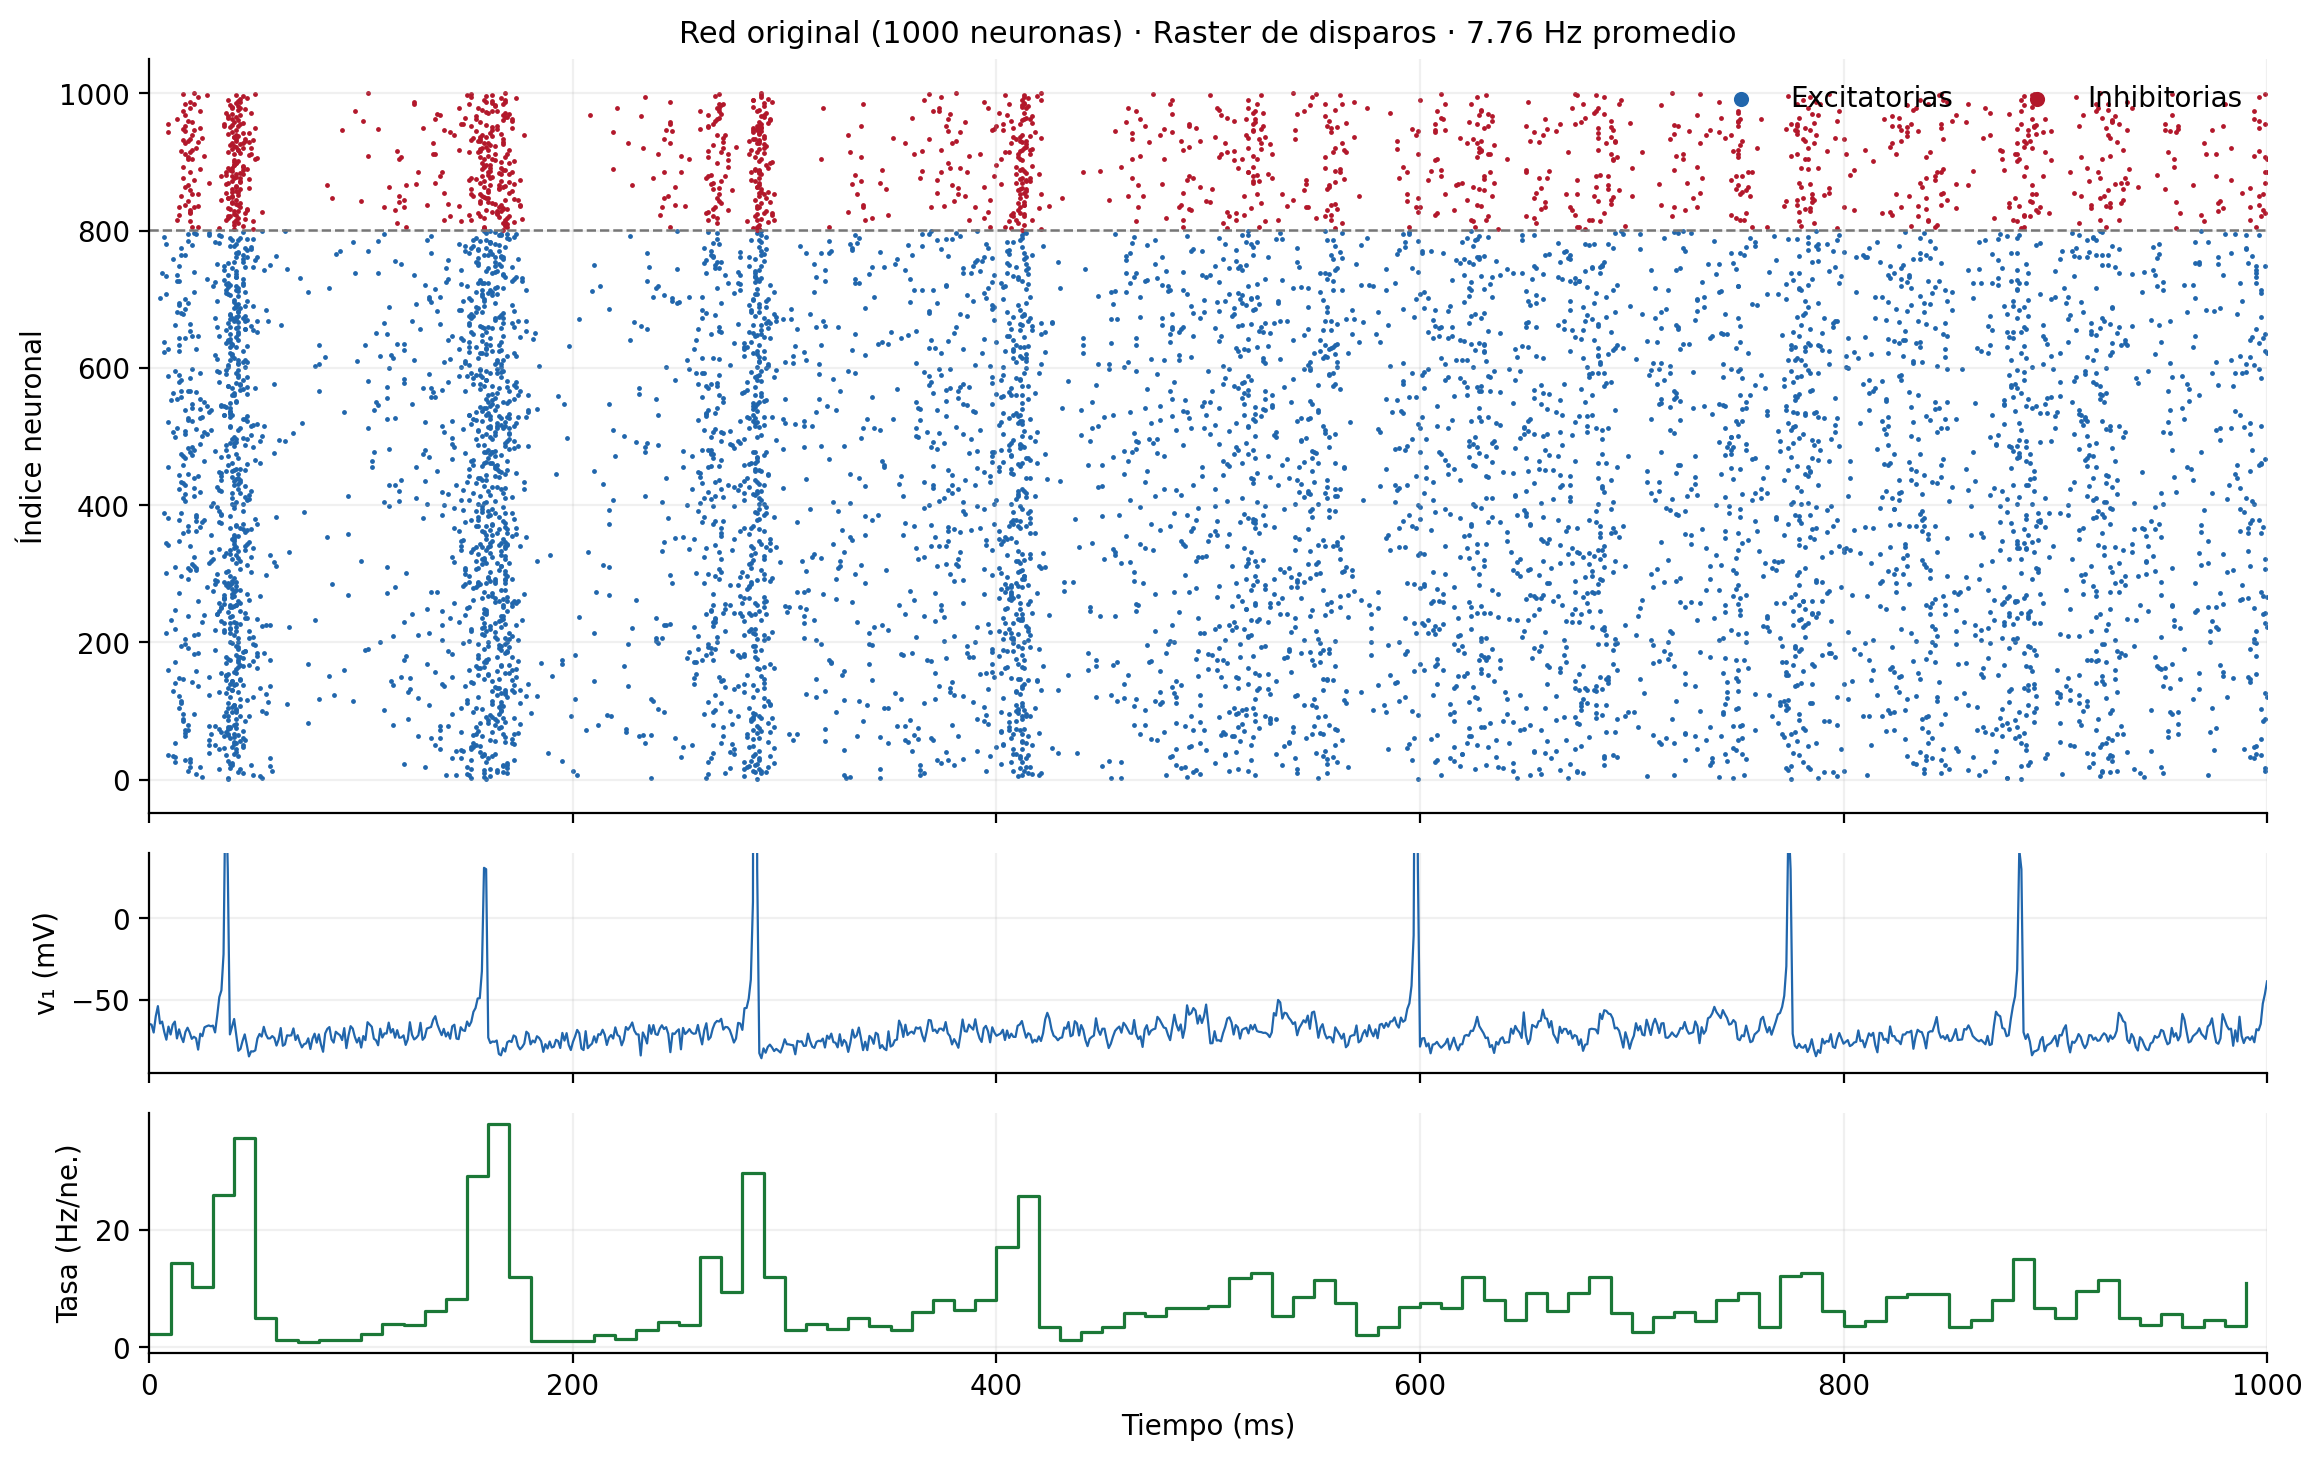
\includegraphics[width=0.78\linewidth]{../figuras/04_red_original.png}
\caption{Red original con autoconexiones: raster excitatorio/inhibitorio, potencial de una neurona y tasa poblacional en ventanas de 10 ms.}\label{fig:red}
\end{figure}
\vspace{-8pt}
En la Fig.~\ref{fig:red} predominan spikes dispersos, interrumpidos por alineamientos verticales (episodios colectivos de sincronización). La tasa media observada fue $7.765$ Hz por neurona, cercana a los $\sim8$ Hz reportados por \cite{izhikevich}, sin atribuirle frecuencias precisas a los episodios únicamente por inspección visual.
\begin{figure}[h!]
\centering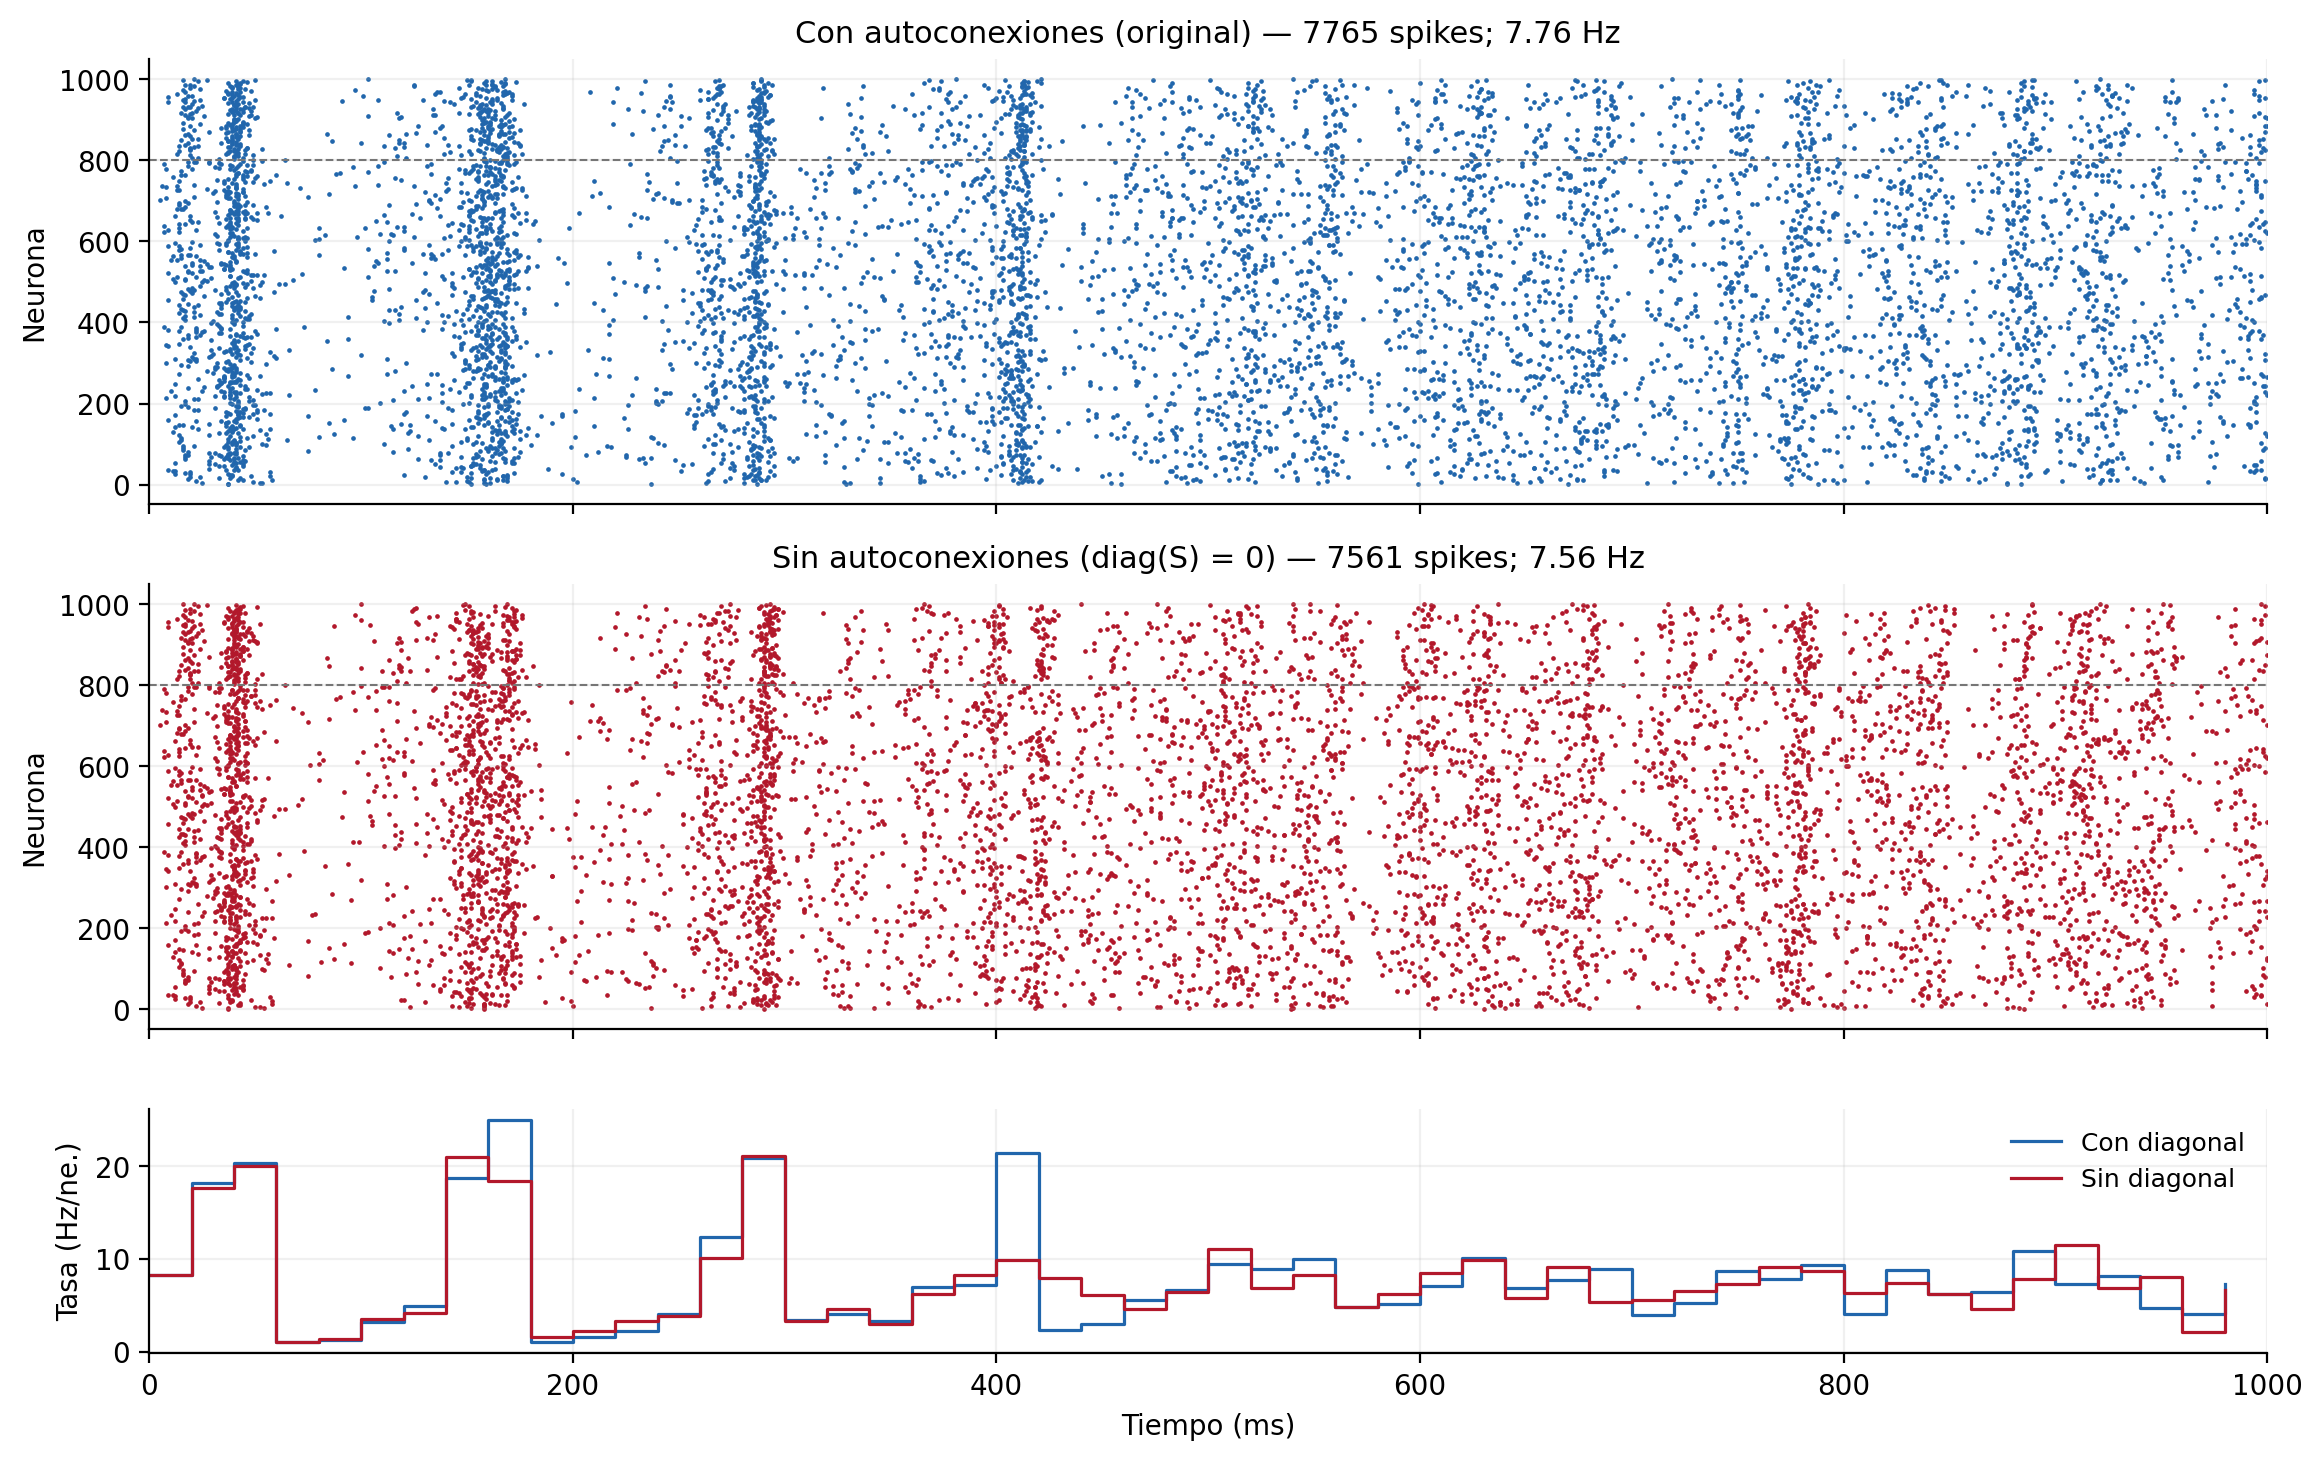
\includegraphics[width=0.75\linewidth]{../figuras/05_red_con_sin_autoconexiones.png}
\caption{Comparación pareada: arriba la matriz $S$ literal; abajo $s_{ii}=0$; tercer panel, tasas en intervalos de 20 ms. Se reutilizaron parámetros, pesos extradiagonales y entradas aleatorias.}\label{fig:comp}
\end{figure}
\vspace{-9pt}
Al suprimir sólo la diagonal, el total pasa de $7765$ a $7561$ spikes ($7.765\to7.561$ Hz): una diferencia de $-2.63\%$. La estructura colectiva general persiste (Fig.~\ref{fig:comp}), aunque divergen eventos y fluctuaciones puntuales; el sistema no es idéntico trayectoria a trayectoria.
\newpage
\section{Ruido continuo y discretización}
Para distinguir el ruido talámico discreto del artículo de una ecuación diferencial estocástica, estudiamos \emph{una sola neurona} con
\begin{equation}
 dV=[0.04V^2+5V+140-U+I(t)]\,dt+\sigma\,dW_t,\qquad dU=a(bV-U)\,dt.
\end{equation}
Integramos localmente mediante Euler--Maruyama: $\Delta V=f(V,U,t)h+\sigma\sqrt{h}\,\xi$, $\Delta U=a(bV-U)h$, con $\xi\sim\mathcal N(0,1)$ independiente y reseteo después de cada paso. Se tomó $h=0.01$ ms, $\sigma=5$ y el escalón de la primera parte; $\sigma=0$ recupera Euler determinista. El factor $\sqrt{h}$ corresponde a incrementos de Wiener y \emph{no} debe introducirse artificialmente en el código discreto original de la red.
\begin{figure}[h!]
\centering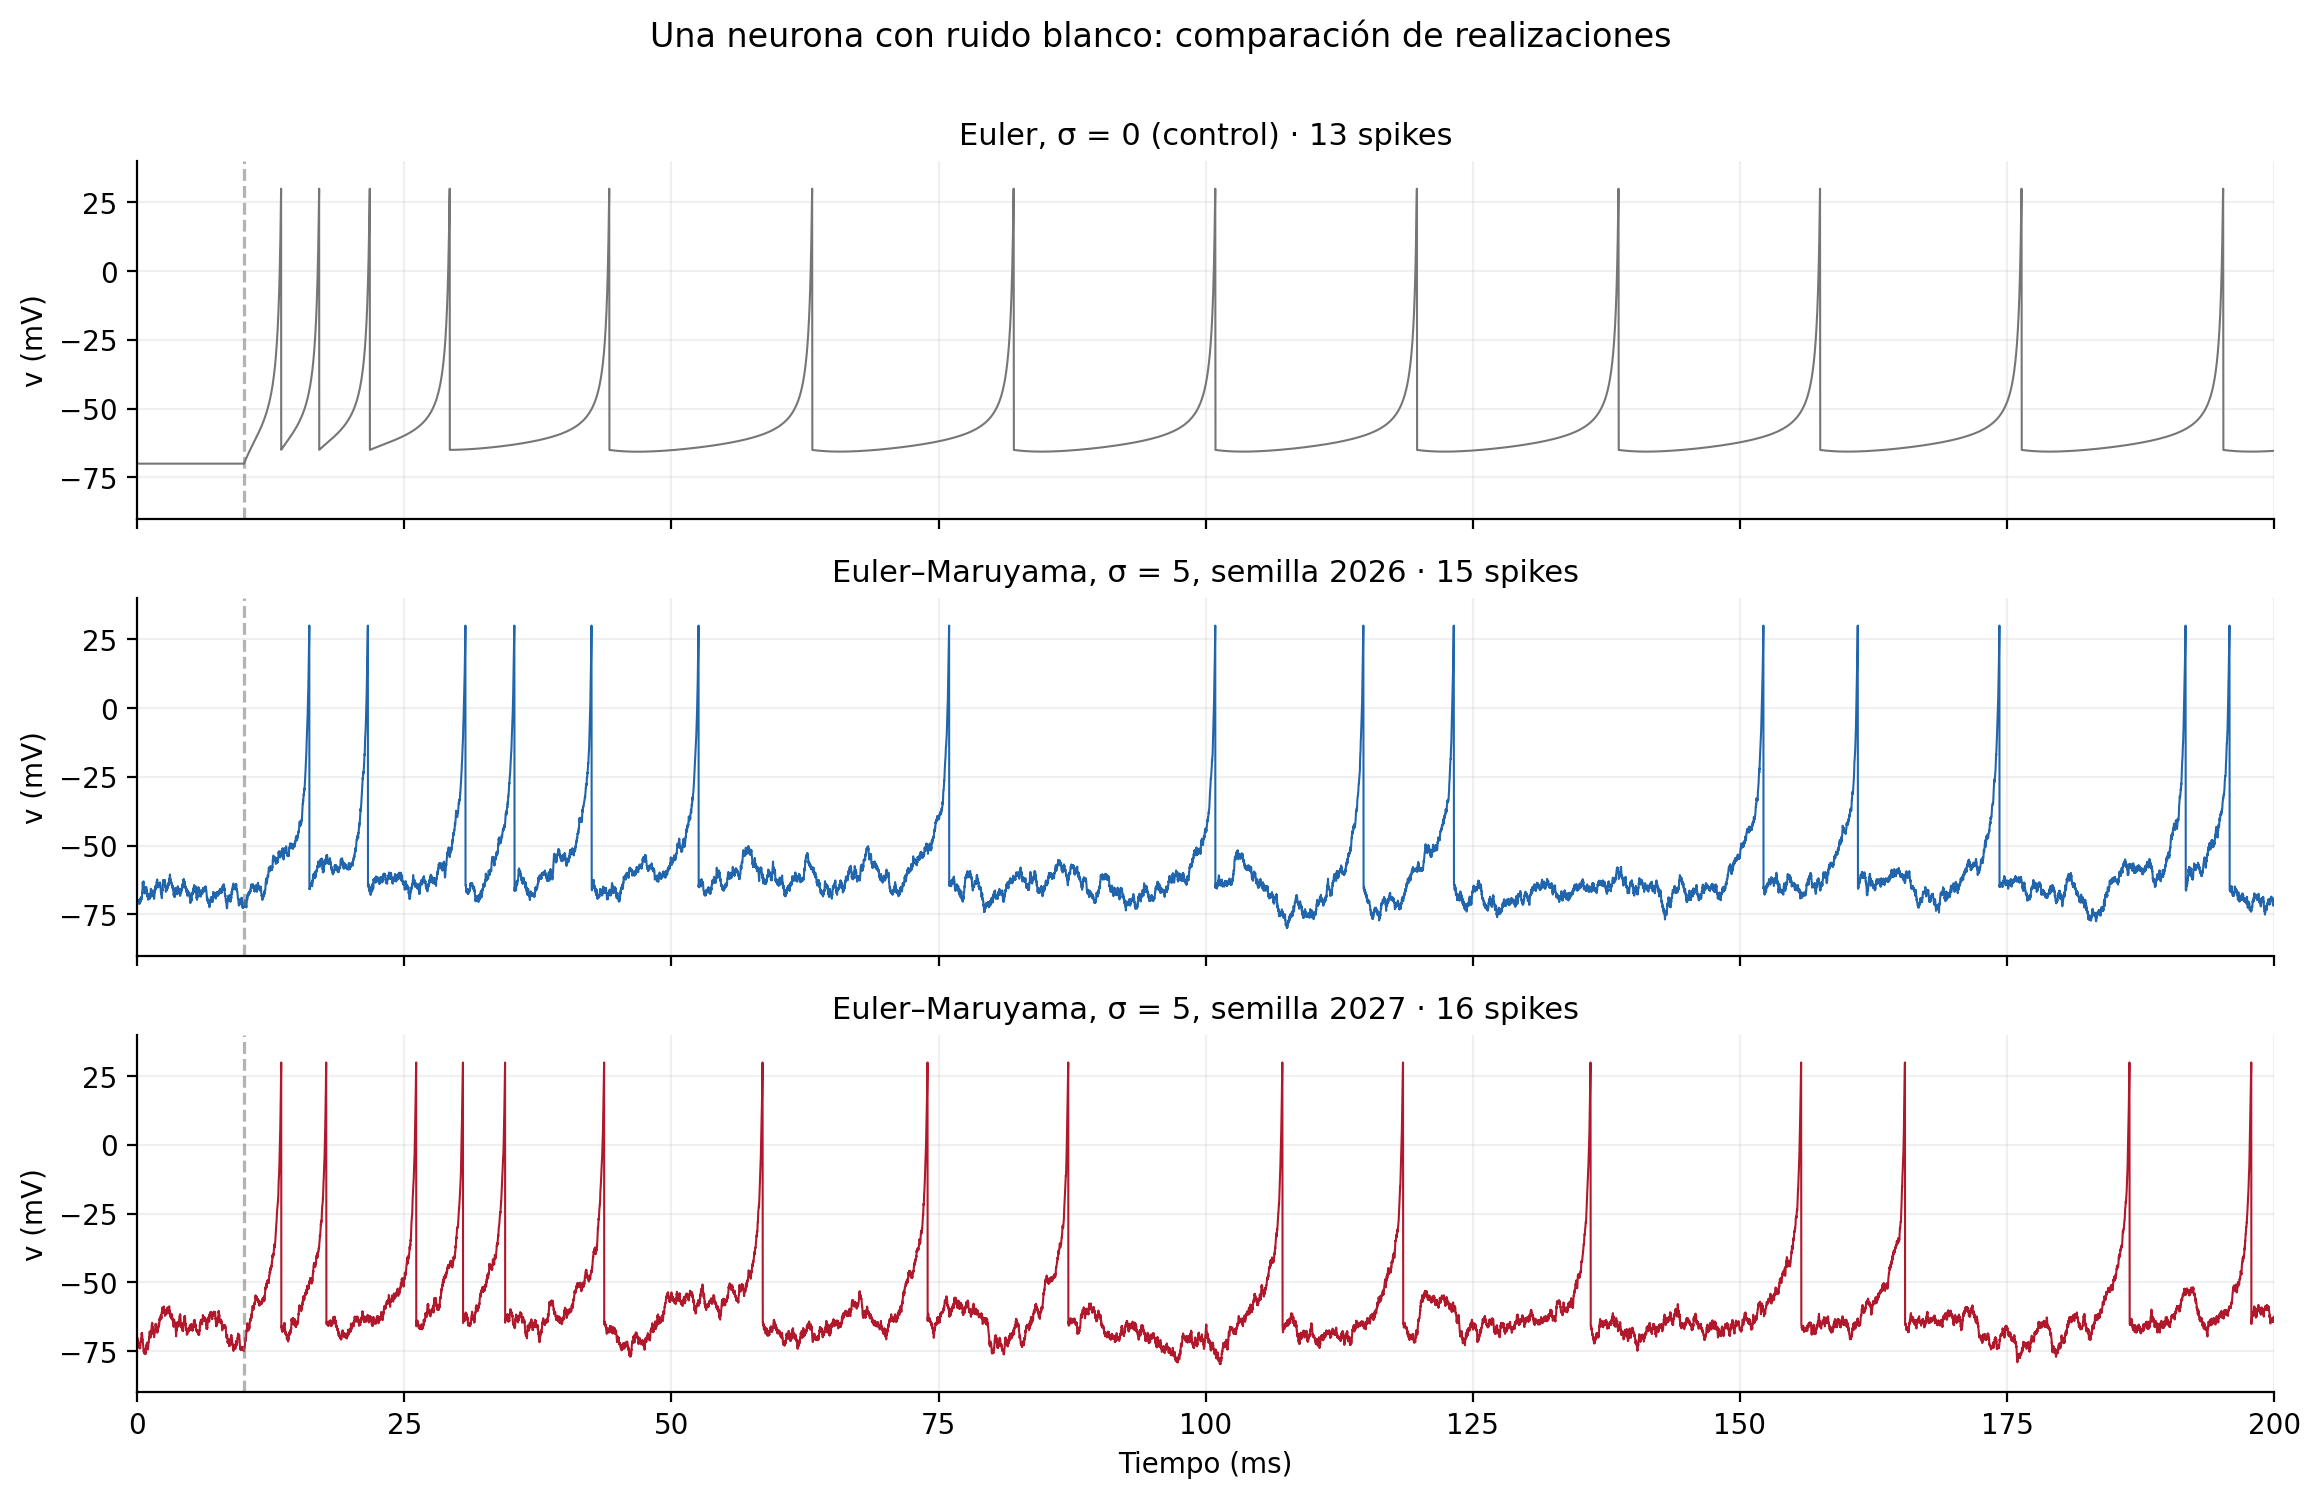
\includegraphics[width=0.73\linewidth]{../figuras/06_una_neurona_ruido_euler_maruyama.png}
\caption{Euler determinista (13 disparos) y dos realizaciones estocásticas independientes: semillas 2026 (15 disparos) y 2027 (16 disparos), $0\!\le t\!\le200$ ms.}\label{fig:ruido}
\end{figure}
\vspace{-5pt}
El ruido modifica la latencia y los intervalos entre spikes sin alterar la regla de reinicio. La variación entre semillas evidencia que el tren de disparos es una \emph{realización}, no una curva determinista.
\begin{figure}[h!]
\centering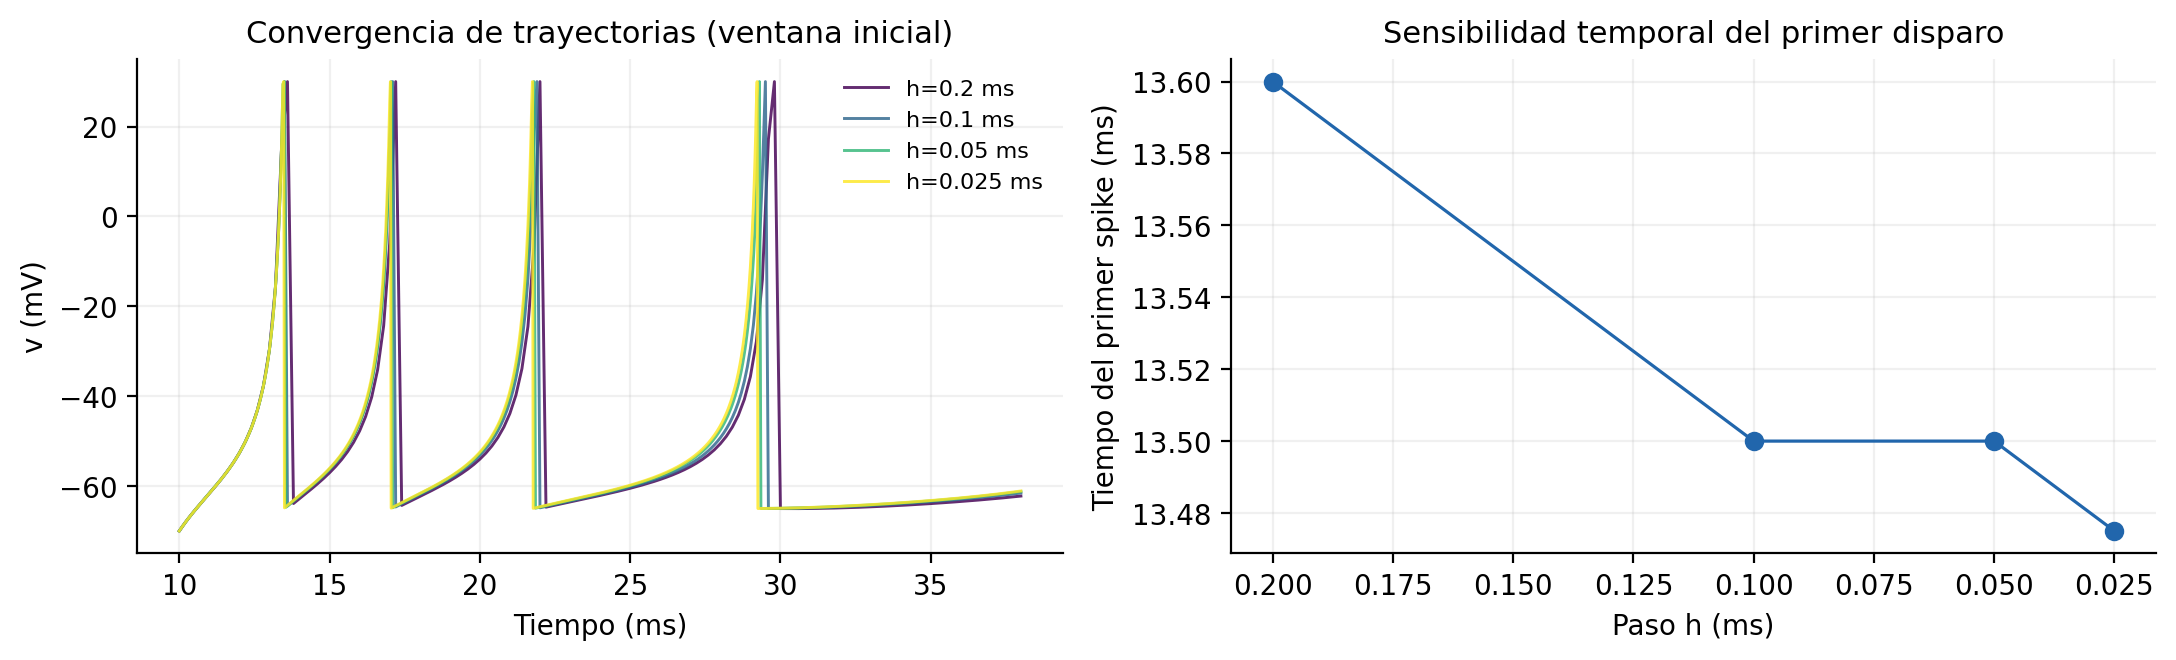
\includegraphics[width=0.68\linewidth]{../figuras/03_sensibilidad_paso.png}
\caption{Sensibilidad del caso base al paso de RK4. Los instantes de reseteo se cuantizan a múltiplos de $h$.}\label{fig:h}
\end{figure}
\vspace{-8pt}
\section{Discusión y conclusiones}
La comparación con la Fig.~2 original es cualitativamente consistente; la red reproduce la actividad media del artículo, no su raster exacto (aleatoriedad diferente). Disminuir $h$ cambia levemente el tiempo del primer spike (Fig.~\ref{fig:h}), porque un reseteo \emph{post-paso} detecta eventos en una grilla; el orden formal cuatro de RK4 entre eventos no garantiza orden cuatro para los tiempos de disparo. También influyen la magnitud del ruido, la topología sináptica y el esquema de integración seleccionado.

{\footnotesize
\begin{thebibliography}{9}\setlength{\itemsep}{-3pt}
\bibitem{izhikevich} E. M. Izhikevich, ``Simple Model of Spiking Neurons,'' \emph{IEEE Transactions on Neural Networks}, vol. 14, n.º 6, pp. 1569--1572, 2003, doi: 10.1109/TNN.2003.820440.
\bibitem{hodgkin} A. L. Hodgkin y A. F. Huxley, ``A Quantitative Description of Membrane Current and Its Application to Conduction and Excitation in Nerve,'' \emph{J. Physiol.}, vol. 117, pp. 500--544, 1952.
\end{thebibliography}}
\end{document}
